\section{Results}

[SOMETHING ABOUT THE SAMPLE THE APPROACH WAS APPLIED TO, I HAD THIS BEFORE BUT WAS CUT OUT IN EDITING]

\begin{figure}
	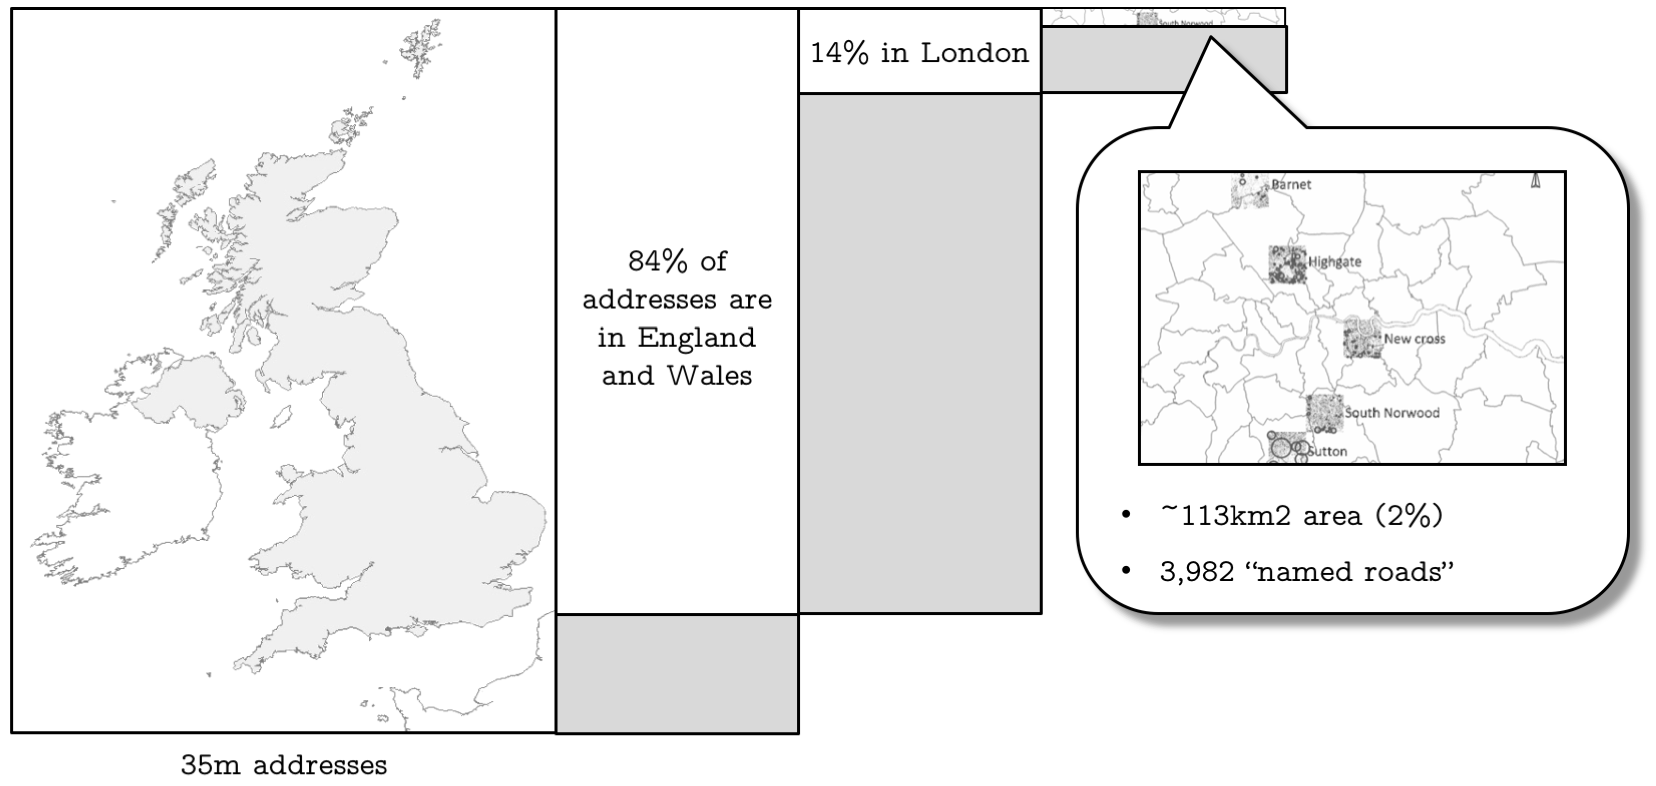
\includegraphics[width=1.0\textwidth]{scope.png}
	\caption{Scope for the experiments}
	\label{fig:scope}
\end{figure}

\subsection{House number inference}

The implementation of the approach described in section \ref{crowdsourcing-olaf} showed that LRPP offers house numbers for 82\% of the streets in scope. The algorithms described in \ref{inference-algorithms} can be applied to the 74\% of roads, generating ~113k house numbers. 

\begin{figure}
	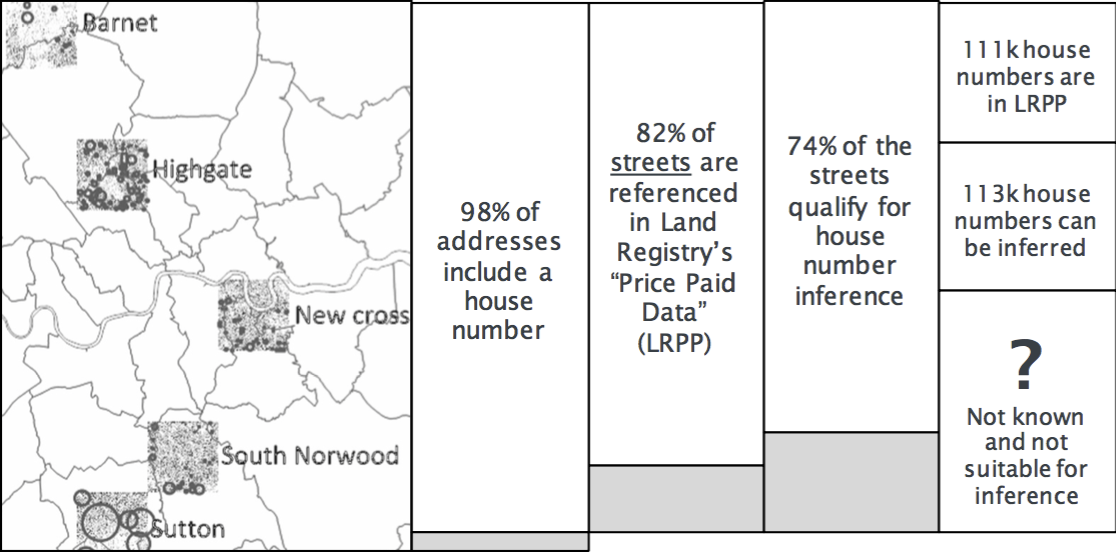
\includegraphics[width=1.0\textwidth]{social-machine-mix-2.png}
	\caption{Primary and derived datasets used to implement the workflow}
	\label{fig:workflow_1}
\end{figure}

\subsection{BLAH}

The result of the experiment is summarised in tables \ref{table:distribution-of-workers} and \ref{table:judgements-summary} below. 

After three consecutive iterations and a total of 150 judgements per road by 80 Workers, the number of total duplicate judgements by reliable Workers was higher than the number of unique judgements, hence triggering the stop condition. 

18.75\% of Workers failed the simple test of copying the name of the road in the form, and were not considered trustworthy. 

Agreement could be reached on four streets only at the end of those three rounds. All roads were identified as not having house numbers.

Collection was reprised at a later point in time to attempt leveraging a different Worker base, through three additional rounds. The judgements of 41 additional Workers were collected, achieving consensus on three more roads. 

\begin{table}[]
\centering
\begin{tabular}{|l|c|c|l|l|}
\hline
                   & \multicolumn{1}{l|}{\begin{tabular}[c]{@{}l@{}}Tot. no. of \\ Workers\end{tabular}} & \multicolumn{1}{l|}{\begin{tabular}[c]{@{}l@{}}No. of new \\ Workers\end{tabular}} & \begin{tabular}[c]{@{}l@{}}No. of \\ reliable\\ Workers\end{tabular} & \begin{tabular}[c]{@{}l@{}}\% of \\ reliable \\ Workers\end{tabular} \\ \hline
First three rounds & 80                                                                                  & -                                                                                  & 65                                                                   & 81.25\%                                                              \\ \hline
All six rounds     & 121                                                                                 & 41                                                                                 & 97                                                                   & 80.16\%                                                              \\ \hline
\end{tabular}
\caption{Distribution of Workers across rounds}
\label{table:distribution-of-workers}
\end{table}



\begin{table}[]
\centering
\begin{tabular}{|l|l|l|l|}
\hline
                   & \begin{tabular}[c]{@{}l@{}}No. of \\ reliable\\ Workers\end{tabular} & \begin{tabular}[c]{@{}l@{}}No. of non-duplicate\\ judgements\end{tabular} & \begin{tabular}[c]{@{}l@{}}No. of roads\\ where consensus\\ was achieved\end{tabular} \\ \hline
First three rounds & 65                                                                   & 117                                                                       & 4                                                                                     \\ \hline
All six rounds     & 97                                                                   & 227                                                                       & 7                                                                                     \\ \hline
\end{tabular}
\caption{Judgement numbers and consensus summary}
\label{table:judgements-summary}
\end{table}

The graph below illustrates how Fleiss kappa variated...

\begin{figure}[!ht]
    \begin{floatrow}
        \ffigbox{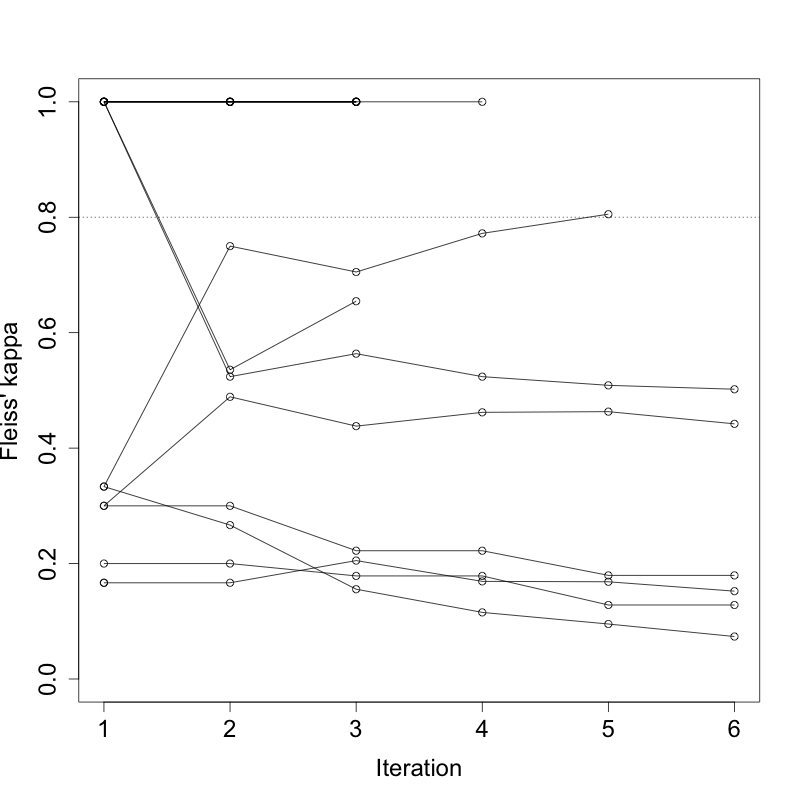
\includegraphics[width=0.5\textwidth]{results-lowest-not-found.png}}{\caption{Roads for which the house numbers were not found. Submissions for the lowest house number.}\label{fig:results-lowest-not-found}}
        \ffigbox{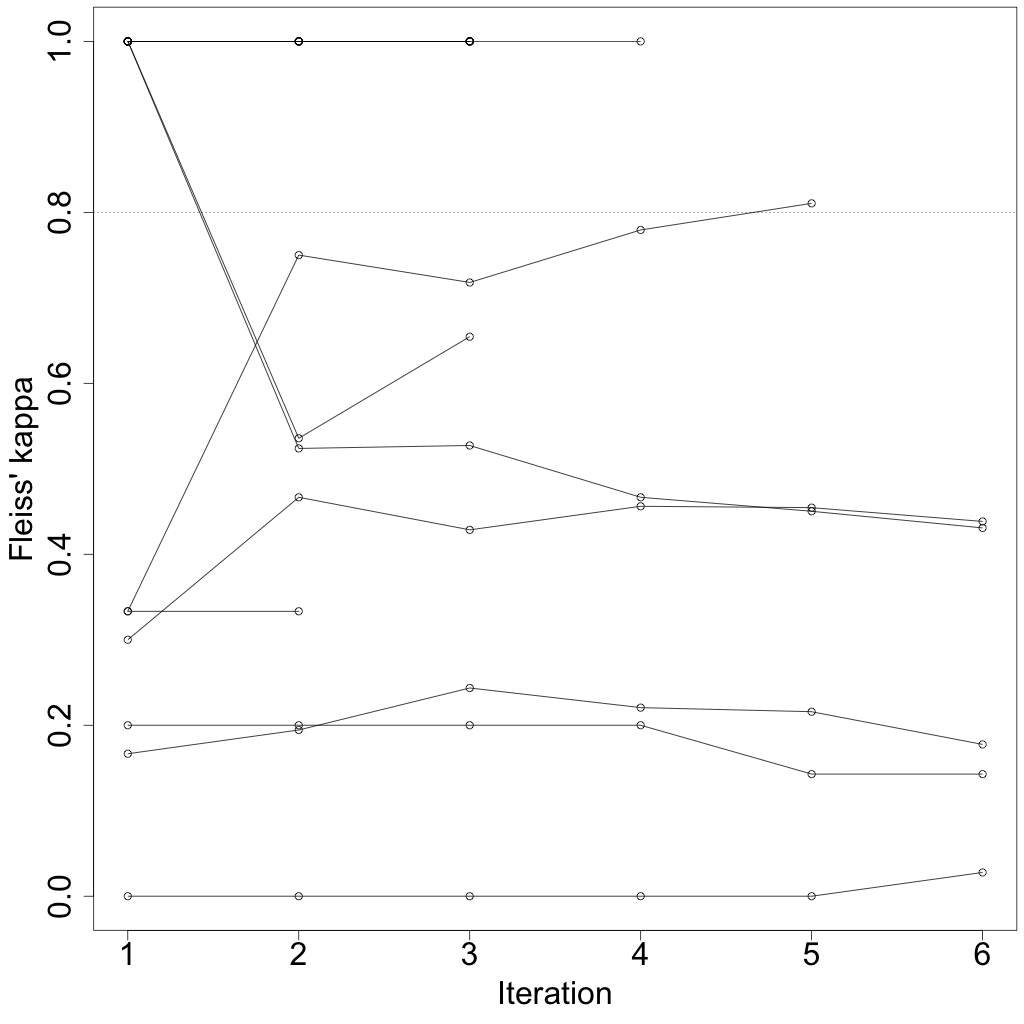
\includegraphics[width=0.5\textwidth]{results-highest-not-found.png}}{\caption{Roads for which the house numbers were not found. Submissions for the highest house number.}\label{fig:results-highest-not-found}}
   \end{floatrow}
\end{figure}
        
\begin{figure}[!ht]
    \begin{floatrow}
        \ffigbox{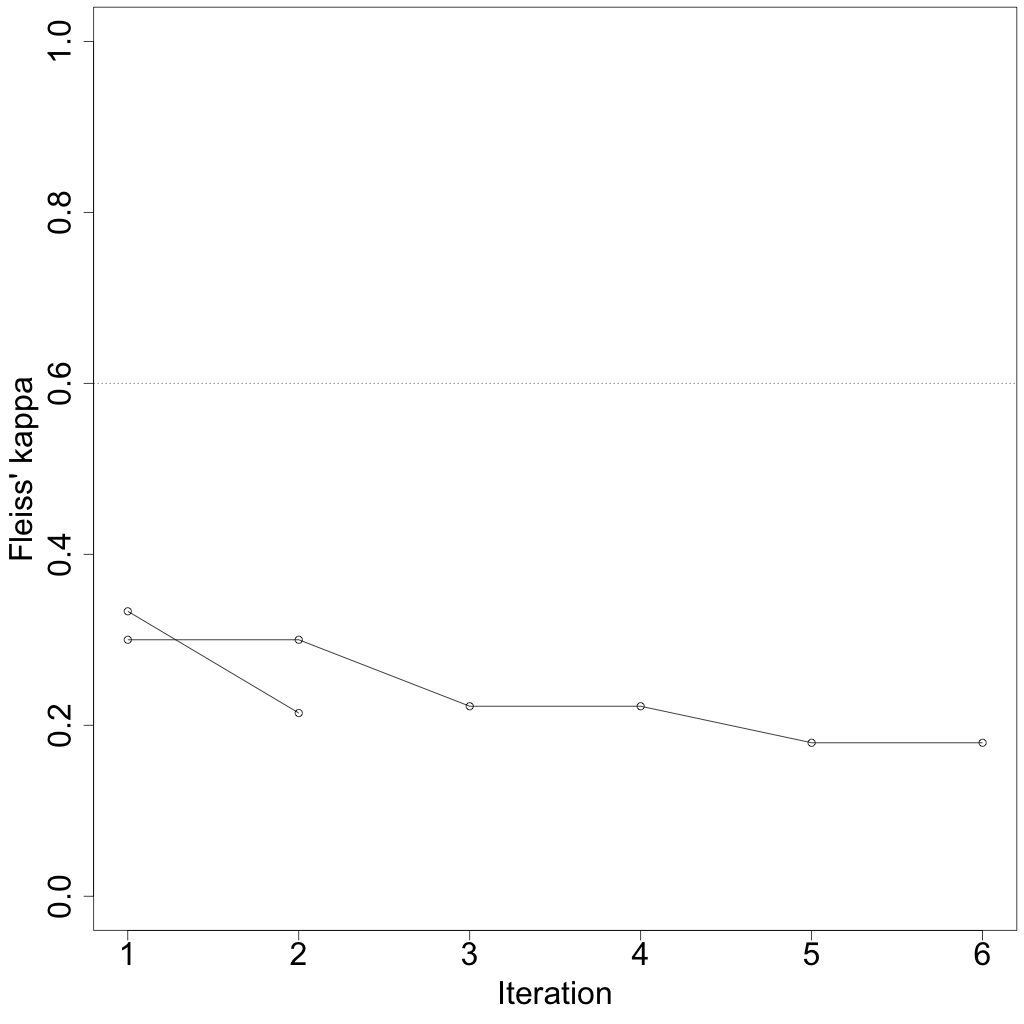
\includegraphics[width=0.5\textwidth]{results-lowest-found.png}}{\caption{Roads for which the house numbers were found. Submissions for the lowest house number.}\label{fig:results-lowest-found}}
        \ffigbox{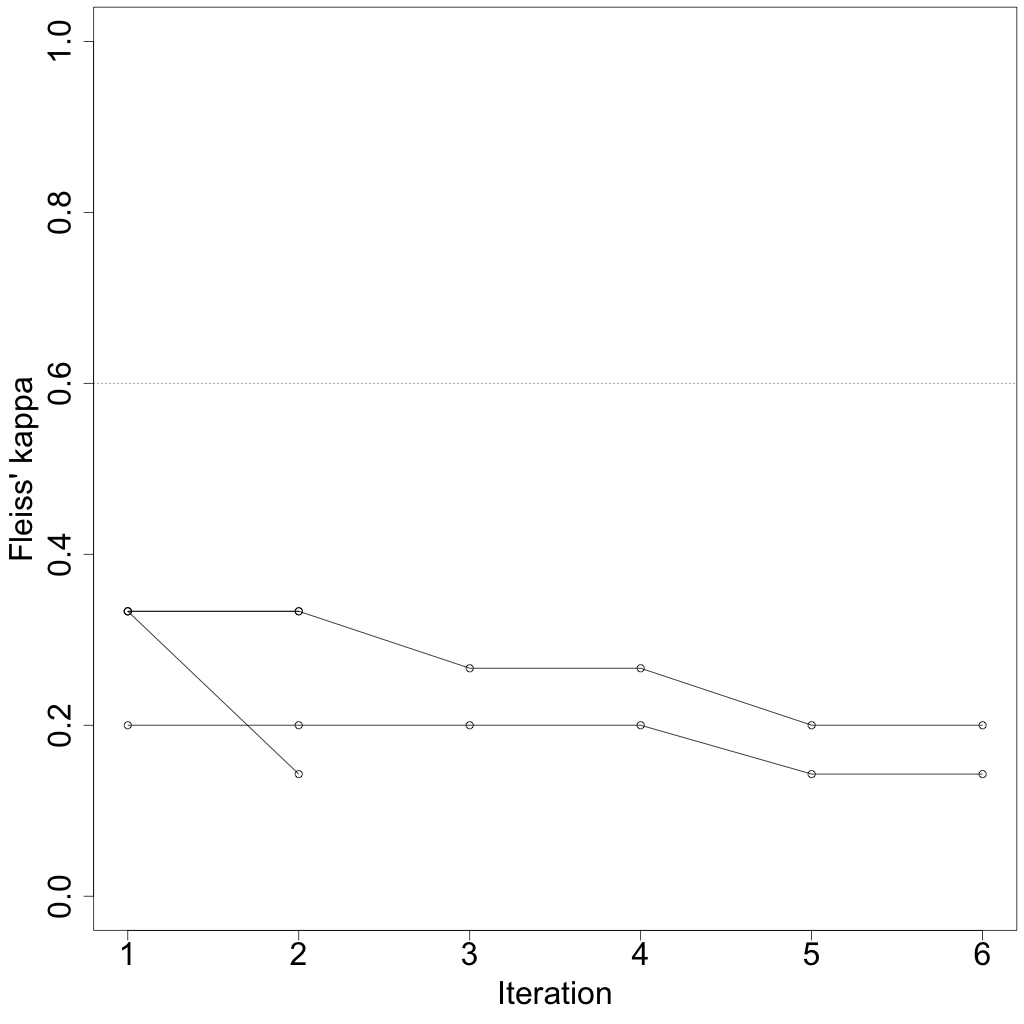
\includegraphics[width=0.5\textwidth]{results-highest-found.png}}{\caption{Roads for which the house numbers were found. Submissions for the highest house number.}\label{fig:results-highest-found}}
   \end{floatrow}
\end{figure}
        